\scanpage{38}
\mspage{\handwritten{6}}
% archive sheet number: 37

\margin{\handwritten{\figure{
\begin{tikzpicture}[scale=.75]
\node[rotate=25,inner sep=1pt] at (0,0) {intervertir};
\draw[rotate=25] (0,0) ellipse (1.05 and .27);
\end{tikzpicture}}}}
Etant donné que les $\handwritten{\unsure{\mathscr{A}|\mathcal{A}}}_i$ sont des anneaux \deleted{\unsure{pas}} nœ thériens, cela permet dans de nombreux\inserted{\handwritten{cas}} de passer
% The typed words retain their positions; the circles and transposition arrow are handwritten.
\figure{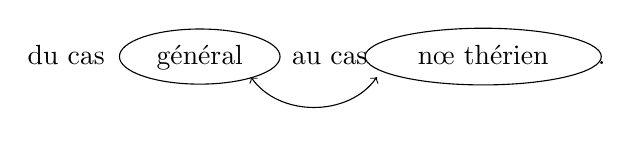
\begin{tikzpicture}
\node[anchor=base east,inner sep=0pt] at (-1.2,0) {du cas};
\node[anchor=base,inner sep=0pt] at (0,0) {général};
\node[anchor=base,inner sep=0pt] at (1.65,0) {au cas};
\node[anchor=base,inner sep=0pt] at (3.6,0) {nœ thérien};
\node[anchor=base west,inner sep=0pt] at (5.05,0) {.};
\handwritten{\draw (0,.10) ellipse (1.02 and .35);
\draw (3.6,.10) ellipse (1.50 and .36);
\draw[<->] (.65,-.16) to[out=-55,in=-125] (2.25,-.16);}
\end{tikzpicture}}

Nous allons maintenant donner deux résultats concernant le cas particulier envisagé en a).

\uline{Proposition 10.11.}- \uline{Soient $S$ un préschéma intègre de point générique $\handwritten{\eta}$, $G$ un $S$-groupe de présentation finie, $X$ un $S$-préschéma de présentation finie, $u$ et $v$ deux $S$-morphismes de $X$ dans $G$, $i:H\handwritten{\longrightarrow}G$ et $j:K\handwritten{\longrightarrow}G$ deux monomorphismes de présentation finie. Alors :}

\uline{(i) il existe un ouvert non vide $S'$ de $S$ tel que si on note $G'$ (resp $H'$, resp. $X'$, resp $u'$, resp $v'$) la restriction de $G$(resp. $H$,resp. $X$, resp. $u$,resp. $v$) au-dessus de l'ouvert $S'$ de $S$, le foncteur\deleted{\unsure{s}} $\underline{\operatorname{Transp}}(u',v')$ (resp. $\underline{\operatorname{Centr}}(u')$, $\underline{\operatorname{Centr}}_{G'}H')$ soit représentable par un sous-$S'$-préschéma fermé de présentation finie $T'_1$ (resp. $C'_1$, resp. $C'_2$) de $G'$.}

\uline{(ii) supposons que $K_{\handwritten{\eta}}$ soit fermé dans $G_{\handwritten{\eta}}$ (ce qui est le cas si $K$ est un sous-$\deleted{p}S$-préschéma en groupes de $G$ (1.4.2)); alors il existe un ouvert non vide $S'$ de $S$ tel que si on note $G'$ (resp. $H'$, resp. $K'$) la restriction de $G$ (resp. $H$, resp. $K$)au-dessus de l'ouvert $S'$ de $S$, le foncteur $\underline{\operatorname{Transp}}_{G'}(H',K')$ (resp. $\underline{\operatorname{Norm}}_{G'}K')$ soit représentable par un sous-$S'$-préschéma fermé de présentation finie $T'_2$ (resp. $N'$) de $G'$.}

\uline{(iii)supposons que $H_{\handwritten{\eta}}$ et $K_{\handwritten{\eta}}$ soient fermés dans $G_{\handwritten{\eta}}$ (ce qui est le cas si $H$ et $K$ sont des sous-préschémas en groupes de $G$ (1.4.2)); alors il existe \inserted{\handwritten{un ouvert}} non vide $S'$ de $S$ tel que si on note $G'$ (resp $H'$, resp. $K'$) la restriction de $G$ (resp. $H$, resp. $K$) au-dessus de l'ouvert $S'$ de $S$, le foncteur $\underline{\operatorname{Transpstr}}_{G'}(H',K')$ soit représentable par un sous-$S'$-préschéma fermé de présentation finie de $G'$.}

Puisque $G_{\handwritten{\eta}}$, $X_{\handwritten{\eta}}$, $H_{\handwritten{\eta}}$, $K_{\handwritten{\eta}}$ sont plats sur le corps $\handwritten{\kappa}(\handwritten{\eta})$, et que
